%% ----------------------------------
%%   Kap04---Realisierung.tex
%% ----------------------------------

%% zeigen, dass das in Kap. 3 beschriebene Konzept auch realisierbar ist und wie

\chapter{Realisierung}
\label{sec:Chapter4}
In diesem Kapitel wird es um die Realisierung und Implementierung des Konzepts aus Abbildung~\ref{fig:Notengenerierung} gehen. Dabei wird eine detailliertere Darstellung der jeweiligen Abläufe geliefert und speziell darauf eingegangen werden, welche Änderungen es in der schlussendlichen Implementierung im Vergleich zum allgemeinen Konzept gibt. Der komplette Ablauf wurde in der Programmiersprache Java geschrieben. Dabei greift die Realisierung aber auf die bereits vorhandene Software mit dem Namen \glqq Memristor Discovery\grqq\,von Knowm Inc. zurück. Diese Software ist Open Source und bietet eine Umgebung zum händischen Testen der von Knowm gelieferten Memristoren über das Analog Discovery Board.

Im Zuge dieser Arbeit wurde diese Software um eine weitere Funktion im Bereich des sogenannten \glqq Board Checks\grqq\,erweitert. Mit dem Button \glqq Check Quality\grqq\,wird die in den folgenden Abschnitten detaillierter beschriebene Kategorisierung und Benotung des ausgewählten Memristors ausgeführt. Der für diese Arbeit implementierte Teil des Programms umfasst den in Abbildung~\ref{fig:Programm} hervorgehobenen Bereich. Neben dem zuvor beschriebenen \glqq Check Quality\grqq\,Button, gibt es noch zwei Auswahlboxen \glqq Newer Generation of Memristors\grqq\,und \glqq Chromium Memristor\grqq. Die erste Auswahlbox muss ausgewählt werden, wenn die Wolfram, Zinn und Chrom Memristoren der neuen Generation kategorisiert werden sollen. Die zweite Auswahlbox muss zusätlich zur ersten ausgewählt werden, wenn von den Memristoren der neuen Generation die Kategorisierung für die Memristoren aus Chrom durchgeführt werden soll. Die folgenden Abschnitte sind nach der Abbildung~\ref{fig:Notengenerierung}
sortiert. Das Kapitel beginnt also mit der Untersuchung des Hysteresen-Loops und einem möglicherweise dazugehörigen Conditioning, arbeitet danach die Themen zur Bestimmung der Formbarkeit, des Thresholds, der Speichergröße und der Lebensdauer ab und endet mit der Berechnung einer konkreten Note für den Memristor. Um die Beschreibung im Folgenden zu vereinfachen, soll außerdem bei einem Tupel von Spannung und Stromstärke aus der Liste der Messwerte immer von einem \glqq Punkt auf der Hysterese\grqq\,die Rede sein.
\begin{figure}
  \centering
    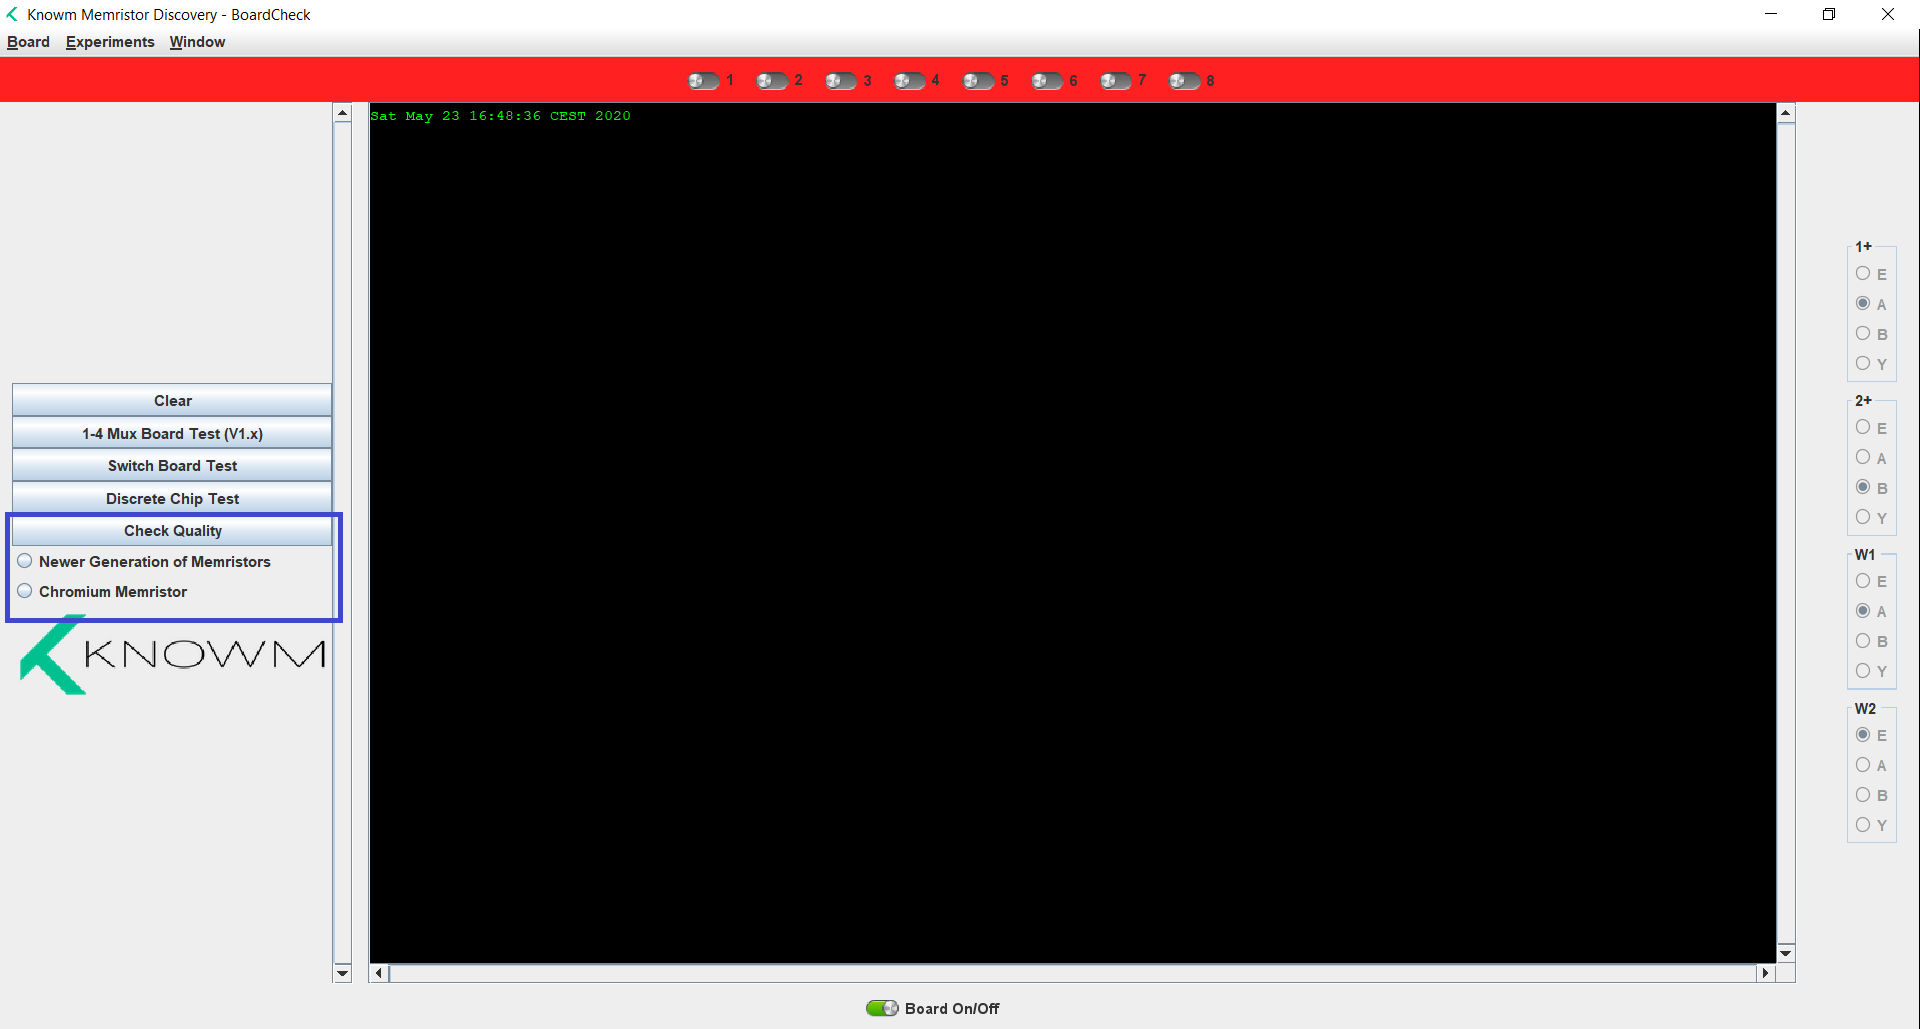
\includegraphics[width=0.9\textwidth]{images/Programm.png}
  \caption{Screenshot des Board Check Interfaces. Blau markiert ist der in dieser Arbeit implementierte Teil}
  \label{fig:Programm}
\end{figure}

\section{Untersuchung der Hysteresen und Bestimmung der Formbarkeit}
Dieser Abschnitt wird den Ablauf der Implementierung zur Bestimmung einer allgemeinen Formbarkeit eines Memristors darstellen. Für die Überprüfung, ob der Memristor überhaupt eine Hysterese besitzt und ob ein Conditioning notwendig ist, wurden feste Parameter gewählt: Eine Frequenz von 100Hz, eine Amplitude von $0.6$V für die Memristoren der alten Generation und $1$V für die Memristoren der neuen Generation und einen Offset von 0. Die Amplituden reichen nach dem Datenblatt von Knowm~\cite{knowm_comp_2019} aus, um bei jedem Memristor den Threshold zu erreichen und darüber hinaus einen Hysteresenbogen zu erhalten. Ein Offset ist für diese Betrachtung nicht notwendig, da dieser nahezu gleiche Bedeutung hätte wie das Anlegen einer höheren Amplitude. Beim Offset wird der Mittelpunkt der Spannungskurve um den Offset verschoben. Die Amplitude bleibt zwar gleich, doch die maximale und minimale Spannung in der Kurve ist um den Offset verschoben. Dabei kann es in einer Richtung nur zu ungenaueren Messergebnissen führen, da dort eine niedrigere Spannung angelegt wird. Der Offset muss in der von Digilent gegebenen Spannungskurve jedoch gegeben werden. Die Frequenz ist nach der Standardeinstellung der Memristor Discovery Software gewählt, um möglichst nah und nachvollziehbar an der in der Software vorhandenen Hysteresendarstellung zu bleiben und ähnliche Messergebnisse zu erhalten.

\begin{figure}
  \centering
    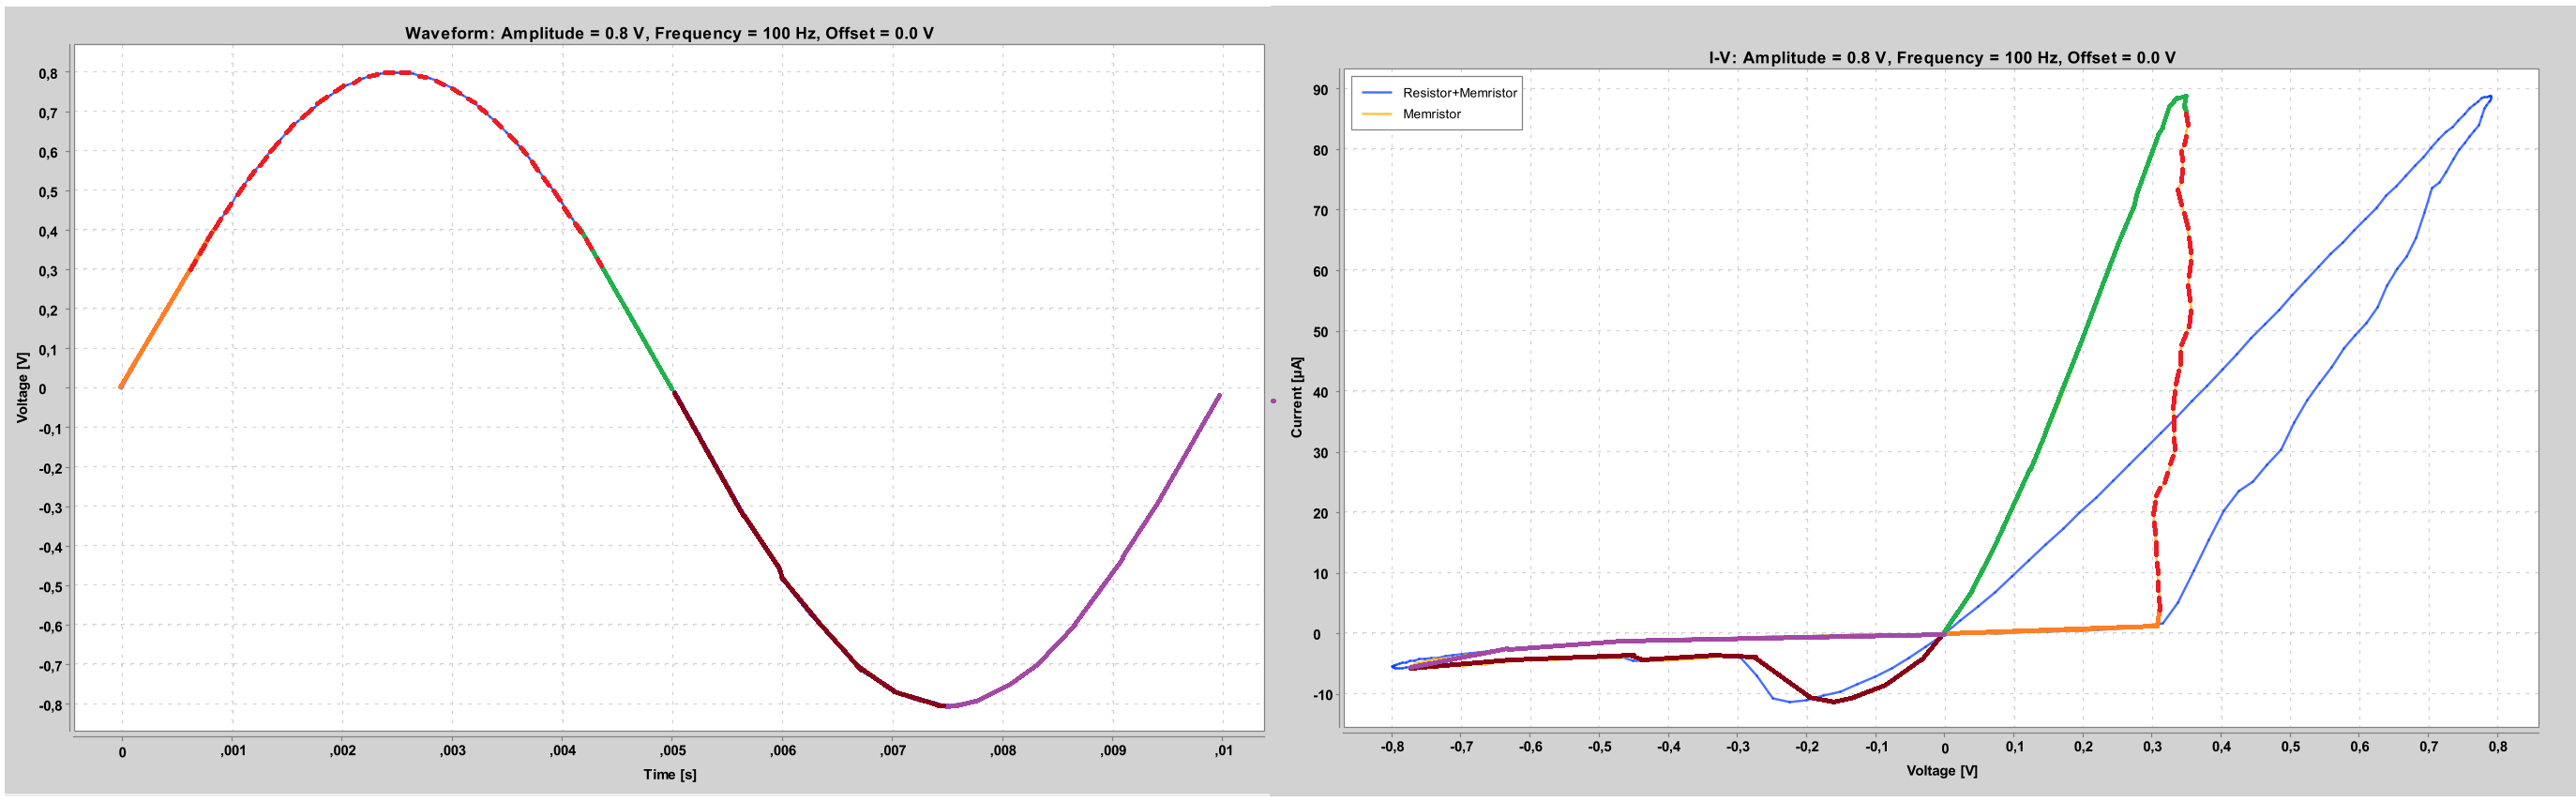
\includegraphics[width=\textwidth]{images/Hysteresen_Split_3.png}
  \caption{Hysteresen Aufteilung anhand der Sinus Kurve der Spannung.}
  \label{fig:Hysteresen_Split}
\end{figure}

Um die Formbarkeit zu messen, muss zu Beginn die Hysterese des ausgewählten Memristors ausgelesen werden. Dafür wird Spannung auf dem ausgewählten Memristor angelegt, welche in Form einer Sinus Kurve alterniert. Ausgelesen wird die Spannung in Volt und die dazugehörige Stromstärke in Milliampere. Ist die Messung abgeschlossen, so liegen die Messwerte als Liste von Tupeln der Form $(V,\mu A)$ vor. Es muss nun erst einmal überprüft werden, ob es sich bei der Messung überhaupt um eine Hysterese handelt oder ob nur Messrauschen eingefangen wurde. Dafür wird die Hysterese wie in Abbildung~\ref{fig:Hysteresen_Split} in vier Teile geteilt. Der erste Teil \glqq $f_1$\grqq\,bildet den ersten Anstieg der Spannung auf dem Memristor ab, bis zu dem Zeitpunkt, an welchem das Maximum der Stromstärke erreicht wurde. Die Funktion \glqq $f_2$\grqq\,stellt den Abfall der Hysteresen von der maximalen Stromstärke bis zum Nulldurchlauf dar. Mit \glqq $f_3$\grqq\,wird danach der weitere Abfall vom Nulldurchlauf bis zum Minimum der Spannungskurve betrachtet. Zuletzt bildet \glqq $f_4$\grqq\,die Steigung vom Minimum zum Nulldurchlauf ab. Diese Aufteilung für die Hysterese wurde gewählt, um die folgenden Betrachtungen zur Bestimmung der Formbarkeit und des Thresholds zu vereinfachen.

\begin{table}
  \centering
  \textbf{W, Sn, C Types}
    \begin{tabular}{|l|l|c|c|c|}
      \hline \textbf{Characteristic}   & \textbf{Condition} & \textbf{Min} & \textbf{Typ} & \textbf{Max} \\\hline
      \textbf{Forward Threshold}& DC / Quasi-static  &      $0.15$V        &      $0.26$V        &    $0.35$V \\\hline
      \textbf{Reverse Threshold}& DC / Quasi-static  &       $-0.27$V       &      $-0.11$V        &  $-0.05$V \\\hline
      \textbf{Cycle Endurance}  & $1.5$Vpp, $500$Hz sine wave, &    $50$M          &       $100$M       &   $5$B \\
                                &  $50$k$\Omega$ series resistor &&&\\\hline
    \end{tabular}

    \textbf{Cr Types}
      \begin{tabular}{|l|l|c|c|c|}
        \hline \textbf{Characteristic}   & \textbf{Condition} & \textbf{Min} & \textbf{Typ} & \textbf{Max} \\\hline
        \textbf{Forward Threshold}& DC / Quasi-static  &      $0.22$V        &      $0.33$V        &    $0.56$V \\\hline
        \textbf{Reverse Threshold}& DC / Quasi-static  &       $-0.66$V       &      $-0.19$V        &  $-0.04$V \\\hline
        \textbf{Cycle Endurance}  & $1.5$Vpp, $500$Hz sine wave, &    $1$M          &       $50$M       &   $100$M \\
                                  &  $50$k$\Omega$ series resistor &&&\\\hline
      \end{tabular}
      \quelle{\cite{knowm_comp_2019}}
  \caption{Parameter (Minimum, Typisch, Maximum) für Forward Threshold, Reverse Threshold und Lebensdauer der verschiedenen Memristor Typen (W: Wolfram, Sn: Zinn, C: Kohlenstoff, Cr: Chrom)}
  \label{tab:Threshold_Lifetime_Params}
\end{table}

Davor muss jedoch noch eine Frage geklärt werden. Wieso wurde für \glqq $f_1$\grqq\,und \glqq $f_2$\grqq\,die maximale Stromstärke gewählt und für \glqq $f_3$\grqq\,und \glqq $f_4$\grqq\,die minimale Spannung? Das lässt sich sehr leicht anhand der Abbildung~\ref{fig:Hysteresen_Vergleich} a) und b) erklären. Zu Beginn der Arbeit lagen nur die Memristoren der alten Generation vor. Die Hysteresen dieser Memristoren sind sehr wenig geweitet und der Threshold ist nicht immer erkennbar (siehe Abbildung~\ref{fig:Hysteresen_Vergleich} a). Für diese Hysteresen reicht es aus, für Maximum und Minimum entweder Spannung oder Stromstärke zu wählen. Beides hätte in diesem Fall die gleiche Aufteilung der Funktionen $f_1$ bis $f_4$ zur Folge. Bei den Hysteresen der neuen Generationen, welche in Abbildung~\ref{fig:Hysteresen_Vergleich} b) zu sehen ist, funktioniert dies jedoch nicht mehr. Würde die maximale Spannung als das Maximum gewählt werden, kann es leicht zu einer fehlerhaften Messung kommen. Das liegt daran, dass bei den Memristoren der neuen Generation nach dem Überschreiten des Thresholds ein sehr viel stärkerer Anstieg der Stromstärke zu verzeichnen ist. Wenn die Spannung ihr Maximum erreicht und wieder abfällt, steigt die Leitfähigkeit des Memristors immer noch weiter, bis der Threshold wieder unterschritten wird. Da somit der Widerstand weiter verringert wird, steigt die Stromstärke weiter, obwohl die Spannung sinkt. Somit wird die maximale Stromstärke nicht unbedingt bei maximaler Spannung erreicht. Gleiches gilt für die andere Richtung. Ist der Reverse Threhold der Spannung erreicht, steigt die gemessene Stromstärke des Memristors an. Die minimale Stromstärke wäre in diesem Fall also nicht der Punkt, an welchem $f_3$ endet, sondern der Punkt, an welchem der Reverse Threshold erreicht wird. Deshalb wird hierbei wieder auf die minimale Spannung als Endpunkt von $f_3$ und Startpunkt von $f_4$ gesetzt.

\begin{figure}
  \centering
    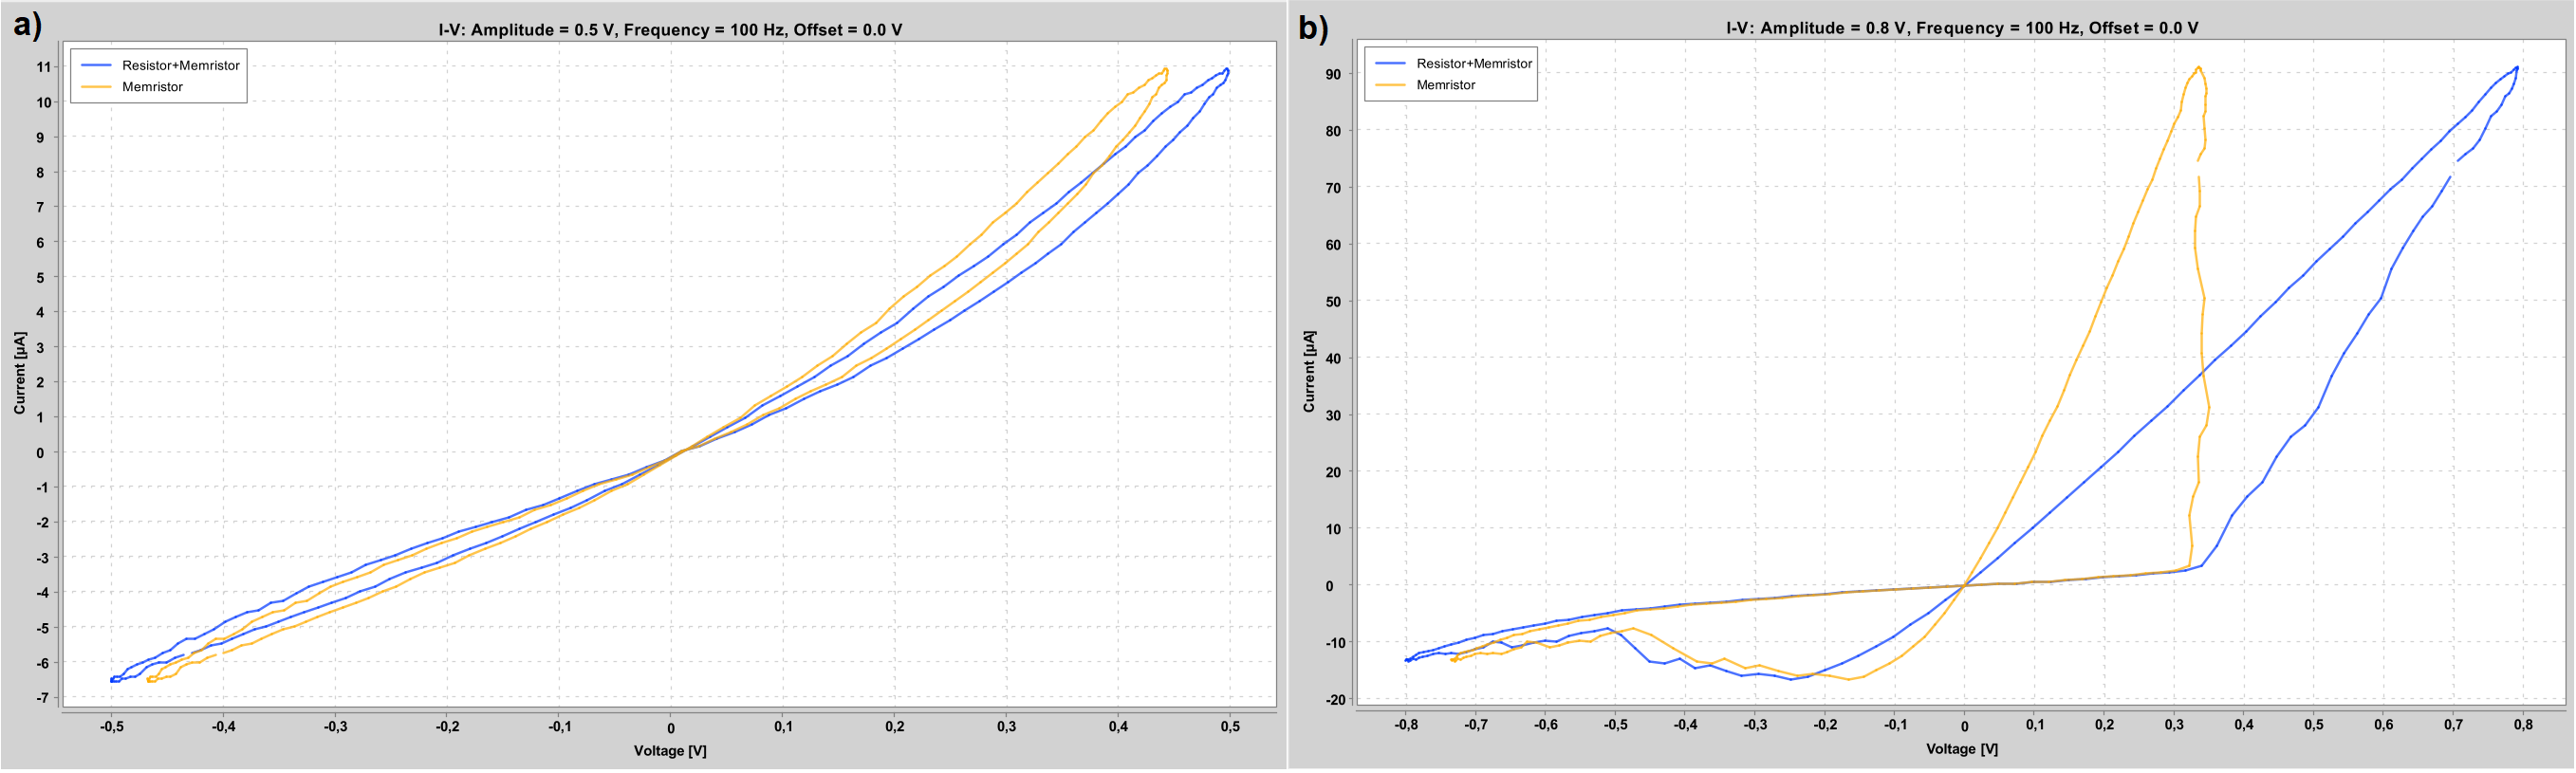
\includegraphics[width=\textwidth]{images/Hysteresen_Vergleich_2.png}
  \caption{Hysteresen a) Memristor der alten Generation b) Memristor der neuen Generation.}
  \label{fig:Hysteresen_Vergleich}
\end{figure}

Es muss zu Beginn überprüft werden, ob die gesammelten Messdaten überhaupt eine Hysterese ergeben. Dafür wird jeder der vier zuvor gebildeten Einzelteile gesondert betrachtet. Die Teile $f_1$ und $f_4$ müssen beide eine durchgehende positive Stromstärke vorweisen, während $f_2$ und $f_3$ eine durchgehende negative Stromstärke besitzen müssen. An dieser Stelle ist anzumerken, dass dieser Test noch nicht erkennt, ob die Hysterese den Charakter einer typischen Hysterese besitzt. Es wird nur ausgeschlossen, dass Messrauschen ohne irgendeine Hysterese in den Messdaten gespeichert wurden. Hat die Hysterese des ausgewählten Memristors nicht einmal diese geprüften Eigenschaften, kann davon ausgegangen werden, dass der Memristor nicht mehr funktionsfähig ist. Er erhält also die Gesamtnote 6, das Programm bricht an dieser Stelle ab. Hält die Messung der Hysterese den geprüften Eigenschaften stand, kann weiter untersucht werden.

Ist dieser Test zu Ende, kann als Nächstes die Notwendigkeit eines Conditionings untersucht werden. Der Test zum Conditioning zusammen mit dem vorherigen Test, welcher Messrauschen ausschließt, stellen hierbei sicher, dass die Messergebnisse die grundlegende Form einer Hysterese haben. Dabei wird der Abstand der Stromstärke in Mikroampere zwischen $f_1$ und $f_2$, sowie zwischen $f_3$ und $f_4$ berechnet und aufaddiert. Einen Grenzwert zu finden, ab welchem ein Memristor ein Conditioning benötigt, erwies sich als schwierig, da die vorhanden Memristoren sehr ähnliche Hysteresen vorwiesen. So sind fast alle Hysteresen der Memristoren auf den Chips der alten Generation von einer eher schlechten Qualität und viele Memristoren auf dem Chip waren bereits zum Zeitpunkt des Starts dieser Arbeit kaputt oder benötigten auf jeden Fall ein Conditioning. Die Hysteresen der Memristoren der neuen Generation haben alle sehr geweitete und schöne Loops. Keine der betrachteten Hysteresen hatte eine merklich schlechtere Qualität als die anderen Hysteresen und selbst die Memristoren, welche lange in Betrieb für Tests und Messungen waren, zeigen immer noch Hysteresen, welche kein Conditioning benötigen.

Nach einige Tests mit verschiedenen Grenzwerten wurden passende Grenzwerte für die Memristoren beider Generationen gefunden. Dabei wurde für die Memristoren der alten Generation darauf geachtet, dass der Grenzwert sie als schlecht oder gerade so akzeptabel kategorisiert. Für die Memristoren der neuen Generation gilt das gleiche, nur dass der Granzwert auf durchschnittliche bis guter Qualität abzielt. Somit ergaben sich ein Grenzwert von 100$\mu A$ für die Memristoren der alten Generation und 500$\mu A$ für die Memristoren der neuen Generation. Dass sich die Werte so weit unterscheiden, liegt unter anderem auch an der höher angelegten Amplitude. Ist die Hysterese nicht genügend geweitet, so wird eine erneute Messung durchgeführt. Davor wird jedoch als Conditioning eine Spannungswelle mit möglichst hoher Amplitude angelegt. Von Knowm wird empfohlen für die Memristoren der alten Generation auf keinen Fall über 1 Volt Spannung anzulegen. Für die Memristoren der neuen Generation gilt dasselbe mit drei Volt Maximum. Für die Memristoren der alten Generation wird vor der erneuten Messung deshalb eine Spannungswelle mit einer Amplitude von 0.95 Volt angelegt, bei den neuen Memristoren liegt die Amplitude bei 2.8 Volt. Die neue Messung, welche nach dem Conditioning durchgeführt wird, muss wieder in vier Teile geteilt werden, wie auch zuvor. Diese Teile können nun erneut darauf untersucht werden, ob es sich um Messrauschen handelt und ob ein Conditioning notwendig ist. Wird erneut ein Conditioning benötigt, so kann davon ausgegangen werden, dass der Memristor selbst mit Conditioning nicht in einen qualitativ hochwertigeren Zustand gebracht werden kann. Das Programm bricht ab und gibt dem Memristor die Note 5, welche für eine sehr schlechte Qualität steht. Hat das Conditioning funktioniert oder ist die Hysterese bereits zum ersten Test geweitet genug gewesen, kann mit dem nächsten Schritt weiter gemacht werden.

\begin{figure}
  \centering
    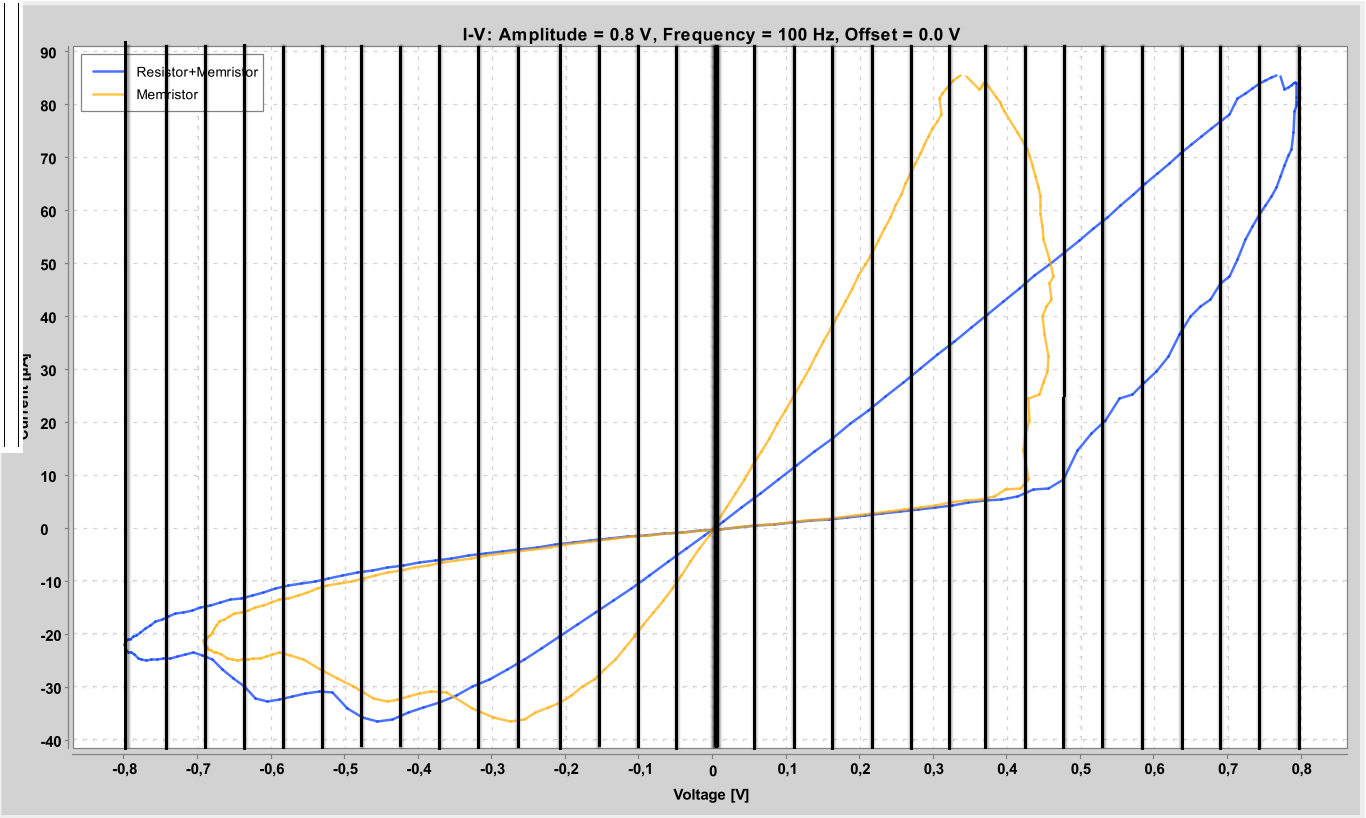
\includegraphics[width=0.8\textwidth]{images/Hysteresen_Sektoren.png}
  \caption{Veranschaulichung der Aufteilung der Hysterese in Sektoren.}
  \label{fig:Hysteresen_Sektoren}
\end{figure}

Nun wird noch einmal die allgemeine Formbarkeit des Memristors untersucht. Dafür werden neun weitere Messungen der Hysterese durchgeführt, für welche unterschiedliche Amplituden gewählt wurden. Die Schritte, mit welchen sich die Amplitude für die Memristoren der alten Generation pro Messung erhöhen, liegt bei $0.05$V. Die Schritte für die neue Generation liegen bei $0.2$V. Die Startwerte der Amplituden sind für die alte Generation $0.4$V und für die neue Generation 0.6V, sodass sich die folgenden Amplituden für die neun Hysteresen ergeben:
\begin{align*}
  &\text{Amplituden}_{neueGen} = (0.6V, 0.8V, 1.0V, 1.2V, 1.4V, 1.6V, 1.8V, 2.0V, 2.2V) \\
  &\text{Amplituden}_{alteGen} = (0.4V, 0.45V, 0.5V, 0.55V, 0.6V, 0.65V, 0.7V, 0.75V, 0.8V)
\end{align*}
Wie zuvor hat der Offset in diesem Fall wieder keinen besonderen Einfluss. Es wird sich also auf die Veränderung der Amplitude konzentriert, weshalb der Offset auf 0 bleibt. Für das Formen eines Memristors in eine bestimmte Form kann der Offset einen großen Einfluss haben, da er die Hysterese in die jeweilige Richtung verschiebt. Für einen allgemeinen Vergleich zwischen den Hysteresen kann der Vergleich jedoch auch einfach durch verschieden hohe Amplituden durchgeführt werden. Ein direkter Vergleich zwischen Hysteresen unterschiedlicher Amplituden ist aber schwierig, da mit verschieden hohen Parametern natürlich auch höhere Abstände zwischen den Hysteresen entstehen und die Position des Threshold an einer anderen Stelle der Hysterese liegt. Bei diesem Vergleich muss jedoch nur auf die Form der Hysteresen geschaut werden.

Dafür wird jede der neun Messungen, wie bei der initialen Messung, wieder in die vier Teile $f_1$ bis $f_4$ aufgeteilt. Jeder dieser vier Teile wird wiederum in 15 gleich große Sektoren aufgeteilt, wie in Abbildung~\ref{fig:Hysteresen_Sektoren} skizzenhaft zu erkennen ist. Jeder Sektor erhält seine Steigung in der Stromstärke, in Abhängigkeit zur angelegten Amplitude als Wert. Im Vergleich der Hysteresen und der Formbarkeit kann nun verglichen werden, was für relative Steigungen die Hysteresen besitzen. Unterscheiden sich diese \glqq genug\grqq, gelten die Hysteresen als unterschiedlich. Genau wie beim Conditioning stellte es sich bei den Memristoren als schwierig heraus, gute Grenzwerte zu finden, ab welchem zwei Hysteresen \glqq unterschiedlich\grqq\,sind. Dafür wurde eine Messreihe gestartet, bei welcher verschiedene Grenzwerte getestet wurden. Dabei wurde der Grenzwert verwendet, bei welchem die Ergebnisse am konsistentesten waren. Am konsistentesten sind Grenzwerte, für welche sehr ähnliche Noten erreicht wurden. Der Grenzwert des Unterschieds der Stromstärkensteigerung zwischen allen 60 Sektoren einer Hysterese eines Memristors mit den Sektoren einer anderen Hysterese liegt nach dieser Messreihe bei 750$\mu A$ für die Memristoren der alten Generation und bei 1900$\mu A$ für die Memristoren der neuen Generation. Unterschreitet der Abstand zwischen zwei Hysteresen diesen Wert, so gelten sie als \glqq zu ähnlich\grqq. Dadurch wird eine der beiden Hysteresen als von der anderen Hysterese \glqq bereits repräsentiert\grqq\,behandelt, was bedeutet, dass kein Vergleich mit dieser mehr notwendig ist, sondern nur noch ein Vergleich mit ihrem Repräsentanten. Die Note für die Formbarkeit bildet sich nach Schema aus Tabelle~\ref{tab:Formbarkeitsnote}. Einfluss dabei hat, wie viele unterschiedliche Hysteresen ein Memristor \glqq formen\grqq\,kann.

\begin{table}
  \centering
    \begin{tabular}{l|c|c|c|c}
      \textbf{Anzahl verschiedener Hysteresen} & $\geq 8$ & $\geq 6$ & $\geq 4$ & sonst \\\hline
      \textbf{Note}          & $1$      & $2$      & $3$      & $4$
    \end{tabular}
  \caption{Verhältnis der Anzahl von verschiedenen Hysteresenformen (von maximal neun) zur Note für die Formbarkeit.}
  \label{tab:Formbarkeitsnote}
\end{table}

\section{Bestimmung der Speichergröße}
Dieser Abschnitt soll sich mit der Implementierung der Bestimmung der Speichergröße beschäftigen. Es muss an dieser Stelle jedoch eine Anmerkung gemacht werden. Obwohl es sich hierbei um das Realisierungskapitel handelt, funktioniert die Bestimmung der Speichergröße in der aktuellen Implementierung nicht. Sie wurde komplett programmiert und getestet, jedoch gibt es Probleme mit der von Knowms Software implementierten Pulserzeugung. Da die Zeit in dieser Arbeit fehlt, um den kompletten Ablauf zur Kategorisierung und Bestimmung des Qualitätsmaßes noch einmal in einem von Knowms Memristor Discovery Software gelösten eigener Implementierung zu erstellen, wurde eine Notlösung implementiert. Da die Pulserzeugung deshalb nicht selbst implementiert werden kann, wird die Implementierung unter der Annahme, dass die Pulserzeugung funktioniert, angegeben und in den folgenden Abschnitten beschrieben. Am Ende dieses Abschnittes findet sich die Beschreibung der Notlösung. Die Implementierung, welche aufgrund der Pulserzeugung nicht funktioniert, jedoch in der Theorie besser funktionieren sollte, wird im Folgenden als der \glqq pulsbasierte Ansatz\grqq\,bezeichnet. Die andere Lösung wird im Folgenden \glqq leitfähigkeitbasierter Ansatz\grqq\,genannt.

Der pulsbasierte Ansatz ist hierbei in zwei Schritte zu unterteilen. Beim ersten Schritt wird der Memristor in den HRS (High Resistive State) gebracht. Der Ablauf würde in der Theorie analog funktionieren, wenn der Memristor zu Beginn in den LRS (Low Resistive State) gebracht wird. In der Implementierung dieser Arbeit wurde entschieden, den HRS als Startpunkt zu wählen, da es sicherer ist, den Memristor in einem hochohmigen Bereich zu nutzen. Memristoren sind in hohen Widerstandsbereichen irgendwann einfach nicht mehr in der Lage, in einen Zustand mit höherem Widerstand zu wechseln, während in niedrigen Widerstandsbereichen in der Theorie keine wirkliche untere Schranke existiert. Der Memristor wird in diesem Fall irgendwann aufgrund des zu niedrigen Widerstandes durchbrennen und nicht mehr funktionsfähig sein. Es wird also aus Vorsicht davor, dass ein Memristor unnötig beim Messen beschädigt wird, zuerst der HRS als Startzustand gewählt.

In den HRS gelangt der Memristor, indem schrittweise durch die vorhandene Software von Knowm der Widerstand in $k\Omega$ wiedergegeben wird und danach durch das Anlegen eines Pulses auf den Memristor versucht wird, in einen höherresistenten Zustand zu gelangen. Beim Puls wird in der Implementierung ein sogenannter \glqq Triangle Pulse\grqq\,genutzt. Unter der Bezeichnung versteht man die Form des Spannungsverlaufs des Pulses, welcher auf dem Memristor angelegt wird. Beispiele für solche Pulsformen finden sich in Abbildung~\ref{fig:Pulsformen}. Die Dreieckform wurde verwendet, da sich hierbei der Bereich, in welchem der Threshold überschritten wird, in einem möglich kleinem Zeitfenster befindet, solange die angelegte Amplitude des Pulses auch dem Threshold entspricht. Somit wird sicher gestellt, dass möglichst kein Zustand \glqq übersprungen\grqq\,wird, da die Weite des Pulses zu groß ist und somit die Thresholdspannung zu lange angelegt wurde. Für die Amplitude des Pulses wird der in den vorherigen Schritten berechnete Reverse Threshold verwendet und um einen festen Wert verringert, damit eine genügend hohe Spannung für den kurzen Moment des Pulses auf dem Memristor liegt, um sich zu verändern. Der Reverse Threshold muss um einen bestimmten Wert verringert werden, damit es überhaupt zu einer Veränderung des Widerstands kommt. Welcher konkrete Wert sich dafür anbietet, müsste durch Messreihen herausgefunden werden, wenn das Pulsen funktioniert.

\begin{figure}
  \centering
    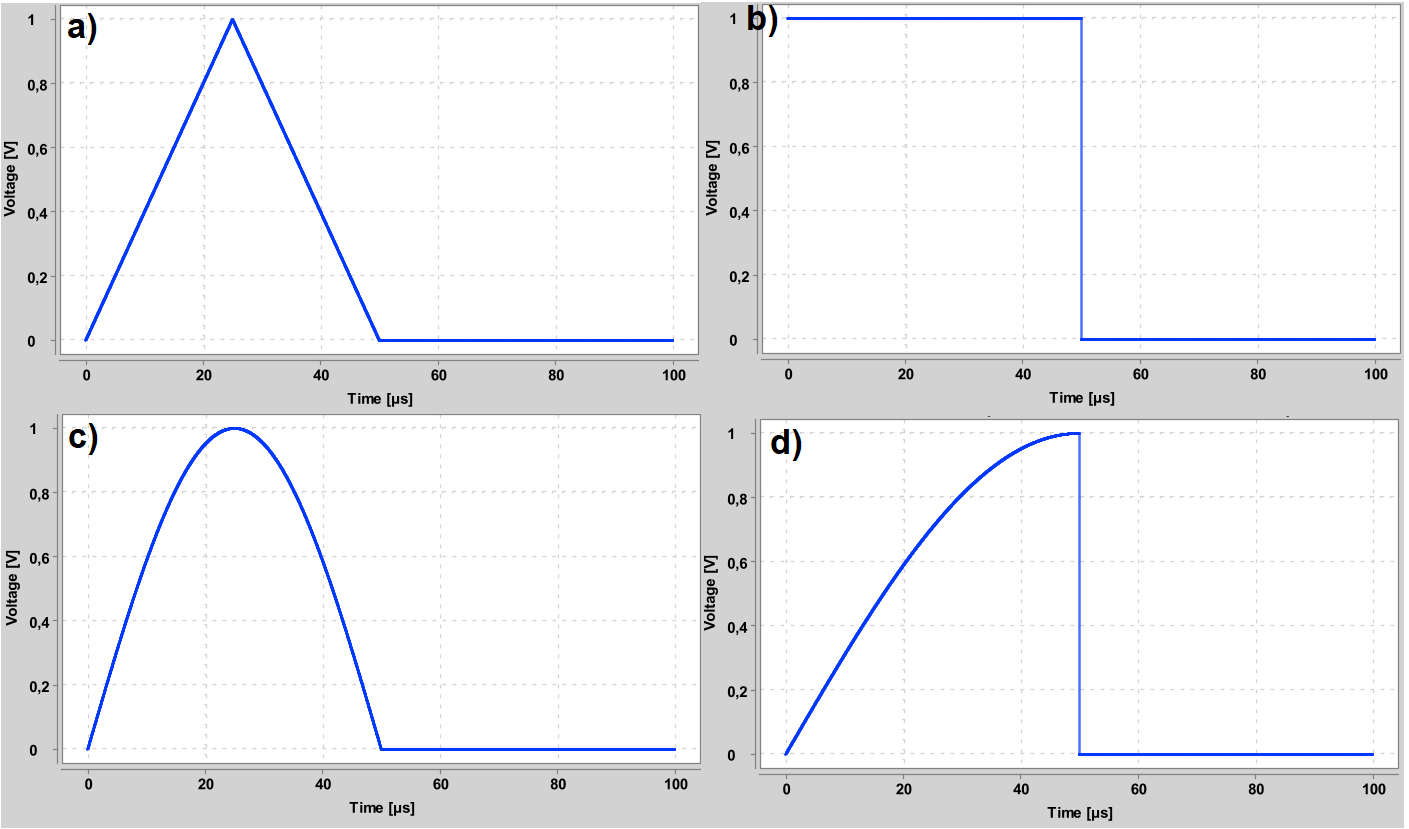
\includegraphics[width=0.85\textwidth]{images/Pulsformen.png}
  \caption{Verschiedene Formen eines Pulses auf einem Memristor: a) Triangle b) Square c) Halfsine d) Quartersine.}
  \label{fig:Pulsformen}
\end{figure}

Nach jedem einzelnen Schritt wird überprüft, ob es sich bei dem zurückgegebenen Widerstand in $k\Omega$ um einen anderen Zustand handelt, welcher noch nicht gefunden wurde. Dabei wird abgefragt, ob der Widerstand um einen bestimmten Grenzwert gestiegen ist. Der Grenzwert muss wieder mit einer funktionierenden Implementierung ausgemessen werden. Ist er nicht gestiegen, so wurde kein weiterer Zustand gefunden.

Ist der Memristor bereits im HRS, kann es in der Praxis manchmal dazu führen, dass der Memristor \glqq umgedreht\grqq\,wird. Dabei wechselt der Forward und Reverse Threshold. Es gibt also noch eine extra Abfrage, ob es beim Anlegen des Reverse Threshold zu einem niedrigeren Widerstand gekommen ist. Ist dies der Fall, wechseln die beiden Thresholds und der HRS wurde gefunden. Verändert sich der Widerstand nach einem Puls gar nicht, so kann auch davon ausgegangen werden, dass der HRS gefunden wurde. Da in so hohen Widerstandsbereichen keine Gefahr besteht, dass der Memristor durchbrennt, wird jedoch, um sicher zu gehen, dass der Puls nicht aus irgendeinem anderen Grund keine Veränderung des Widerstands hervorgerufen hat, vorerst nur ein \glqq Failcounter\grqq\,erhöht. Dabei wird der Puls wiederholt und nur, wenn der Puls wiederholt keine Änderung im Widerstand hervorruft, ist der HRS gefunden.

Der zweite Schritt zur Berechnung der Speichergröße läuft ähnlich zum ersten Schritt ab. Da der Memristor nun im HRS ist, kann durch Pulse der gleichen Form wie im letzten Schritt mit dem Forward Threshold als Amplitude schrittweise ein Zustand nach dem nächsten abgesucht werden. Dabei wird jedoch in jedem Schritt beim Finden eines neuen Zustandes ein Zähler inkrementiert, welcher am Ende die Anzahl der verschiedenen Zustände darstellen soll. Auch hier sollte zur Sicherheit eine Wiederholung des Pulses durchgeführt werden, wenn sich der Memristor noch nicht in einem zu niedrigen Widerstandsbereich befindet und keine Veränderung des Widerstandes gemessen wurde. Es muss jedoch nicht auf das Umdrehen des Memristors geachtet werden, da dies nur im Erhöhen des Widerstandes im hochohmigen Bereich vorkommt. Es kommt aber ein anderer Faktor zur Geltung.

Wie bereits in diesem Abschnitt angesprochen wurde, kann ein Memristor in niedrigen Widerstandsbereichen durchgebrannt werden. Deshalb wird bei jedem Schritt überprüft, ob sich der Memristor nahe des minimalen Widerstandsbereichs der Knowm-Memristoren befindet. Dieser liegt in der Praxis meist bei ungefähr 10 $k\Omega$, nachzulesen im Knowm Datenblatt~\cite{knowm_comp_2019}. Befindet sich der Zustand nahe diesem Widerstandes, so wird nicht weiter nach niedrigeren Widerständen gesucht, da der Memristor im schlechtesten Fall durchbrennen könnte. Dabei kann es natürlich dazu kommen, dass ein möglicher Zustand im niedrigerohmigen Bereich übersehen wird, jedoch sollte vor allem verhindert werden, dass der Memristor beim Testen der Qualität durchbrennt. Verringert sich der Widerstand nach wiederholten Pulsen nicht weiter oder ist der minimale Widerstandsbereich erreicht, kann der LRS festgehalten und der Vorgang zur Bestimmung der Speichergröße beendet werden. Nun liegen drei Parameter vor: Der HRS, der LRS und die Anzahl der verschiedenen Zustände. Aus dem Letzteren lässt sich die Note für die Speichergröße bestimmen, wie in Tabelle~\ref{tab:Speichernote} zu sehen ist. Der HRS und LRS werden nur festgehalten, da diese noch eine Rolle in der Approximation der Restlebensdauer spielen, auf welche im nächsten Abschnitt näher eingegangen wird.

Der folgende Absatz soll nun einmal den leitfähigkeitbasierten Ansatz zur Speichergrößenbestimmung beschreiben, welcher implementiert wurde, da der pulsbasierte Ansatz durch die Memristor Discovery Software nicht funktioniert. In der Memristor Discovery Software von Knowm wurde ein eigenes Puls-Experiment implementiert, in welchem der Nutzer mit händisch eingestellten Parametern Pulse auf ausgewählte Memristoren auf dem Board schicken kann und danach die Leitfähigkeit angezeigt bekommt. Nach diesem Experiment wurde die Leitfähigkeit nach einem Puls ausgerechnet. Da die Leitfähigkeit in Form eines Arrays berechnet wird, ist es nicht wirklich möglich, einen klaren HRS zu bestimmen, wie in der davor beschriebenen Implementierung. Es wird also nur von dem aktuellen Punkt in eine Richtung gepulst, bis keine neuen Leitfähigkeitswerte gefunden wird. Bei Betrachtung des Puls-Experiments kann auch beobachtet werden, dass die Messergebnisse nach dem Schicken eines Pulses sehr stark schwanken, was in einem automatisierten Prozess kaum von einer tatsächlichen Änderung der Leitfähigkeit unterschieden werden kann. Diese Art der Speichergrößenbestimmung ist dementsprechend sehr ungenau und sollte auch in dieser Form nicht in andere Arbeiten übernommen werden.

\begin{table}
  \centering
  \begin{tabular}{l|c|c|c|c|c|c}
    \textbf{Anzahl Zustände}  & $n \geq 16$ & $ 15 \geq n  > 8$ & $8 \geq n > 4$ & $4 \geq n \geq 3$ & $n=2$ & sonst  \\\hline
    \textbf{in Bit}        & $4$       & $3.5$                & $3$                 & $2$  & $1$  & $0$ \\\hline
    \textbf{Note}          & $1$       & $2$                & $3$                 & $4$  & $5$  & $6$
  \end{tabular}
  \caption{Anzahl $n$ an verschiedenen Zuständen im Verhältnis zur Note.}
  \label{tab:Speichernote}
\end{table}

\section{Bestimmung des Energieverbrauch}

Dieses Teilkapitel soll sich mit dem nächsten Schritt der Notengenerierung beschäftigen: Der Bestimmung des Energieverbrauchs. Hier kommt das gleiche Problem aus dem vorherigen Kapitel zu tragen. Da die Pulse nicht funktionieren, ist es nicht möglich, den Memristor bei der Messung sicher in den LRS zu bekommen. Dementsprechend kann der Ansatz aus Kapitel~\ref{sec:Chapter2}, bei welchem LRS und Threshold benötigt werden, nicht fehlerfrei angewandt werden. Dementsprechend wurde der Ansatz gewählt, bei welchem ein konstanter LRS angenommen wird und der Threshold den einzigen Faktor für den Energieverbrauch darstellt.

Da in einem früheren Schritt bereits die Formbarkeit bestimmt wurde, ist es im Weiteren sehr einfach den Threshold auszulesen. Dabei ist Folgendes anzumerken: Wenn im folgenden Teil dieser Arbeit von \glqq dem Threshold\grqq\,die Rede ist, wird dabei impliziert, dass die zwei verschiedenen Thresholds eines Memristors gemeint sind. Dabei handelt es sich einmal um den den sogenannten \glqq Forward Threshold\grqq, welcher den Threshold beim Anlegen einer positiven Spannung darstellt und unter welchem sich der Widerstand des Memristors im Normalfall, wenn er nicht gedreht wurde, verringert. Der andere Threshold ist der sogenannten \glqq Reverse Threshold\grqq, welcher den Threshold beim Anlegen einer \glqq negativen\grqq\,Spannung darstellt. Unter negativer Spannung ist dabei eine positive Spannung in die andere Richtung gemeint. Dabei wird der Widerstand des Memristors erhöht.

\begin{figure}
  \centering
    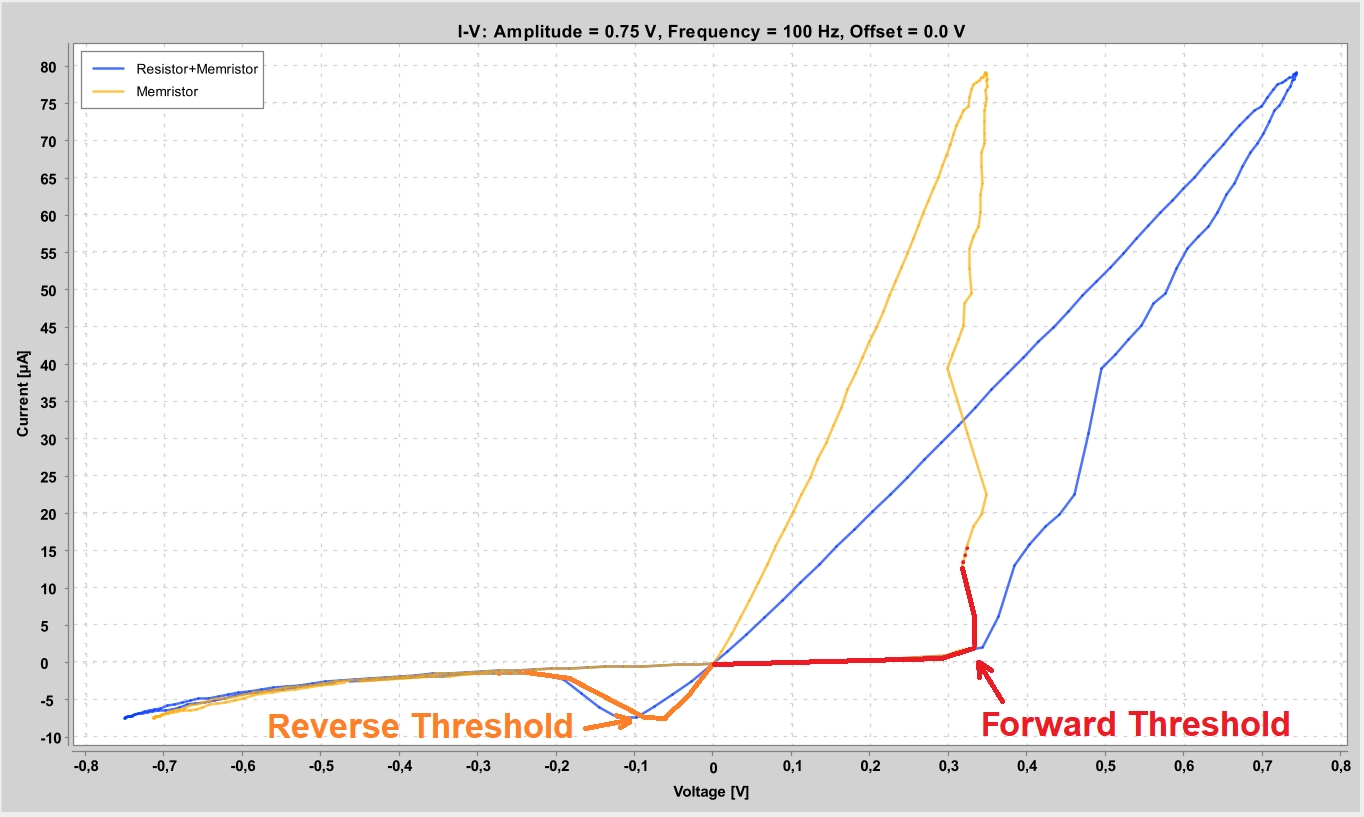
\includegraphics[width=0.8\textwidth]{images/Threshold_Bestimmung.png}
  \caption{Der Forward Threshold kann aus der Teilfunktion $f_1$ ausgelesen werden. Der Reverse Threshold kann aus der Teilfunktion $f_3$ ausgelesen werden.}
  \label{fig:Threshold_Bestimmung}
\end{figure}


Der Threshold lässt sich wie bereits gesagt sehr einfach bestimmen, da bereits vier Teile der Hysteresenfunktion vorliegen. Im Teil $f_1$ lässt sich der \glqq Forward Threshold\grqq\,ablesen, im Teil $f_3$ der \glqq Reverse Threshold\grqq. Die Teilfunktionen $f_1$ und $f_3$ liegen beide in Form einer Liste von Punkten auf der Hysterese vor. Um den Forward Threshold zu bestimmen, wird $f_1$ betrachtet. Da im vorhergegangenen Code bereits überprüft wurde, ob die Funktionen die grundlegenden Eigenschaften einer Hysterese erfüllen, kann in diesem Schritt davon ausgegangen werden, dass $f_1$ eine hysteresentypische Form besitzt. Dementsprechend beginnt $f_1$ mit einem langsamen linearen Wachstum der Stromstärke, von Punkt zu Punkt auf der Hysterese. Sobald der Forward Threshold erreicht ist, beginnt die Stromstärke ein stark erhöhtes Wachstum, wie in Abbildung~\ref{fig:Threshold_Bestimmung} zu erkennen ist.

Es gilt also den Punkt zu finden, bei welcher Spannung für $f_1$ das erhöhte Wachstum der Stromstärke einsetzt. Dabei wird von Punkt zum dem nachfolgenden Punkt auf der Funktion die Steigung der Stromstärke betrachtet. Auch wird der Durchschnitt der Steigung über den gesamten bereits betrachteten Suchraum dargestellt. Ist das Wachstum von einem Punkt zum nächsten um 50\% höher als der Durchschnitt über die aktuelle Steigerung, so ist der Forward Threshold gefunden. Da das Erreichen des Thresholds meistens zu einem exponentiellen Wachstum der Stromstärke führt, liegt es nahe statt 50\% ein Wachstum von 100\% zu suchen. Da die Punkte auf der Messung der Hysterese jedoch sehr nahe beieinander liegen, kann es dazu kommen, dass beim Erreichen des Thresholds das Wachstum zum nächsten Punkt zwar stark steigt, aber noch nicht in einem Schritt um die gesuchten 100\%. Deshalb wurde ein niedrigeres Wachstum angepeilt, da ohne das Erreichen des Thresholds der Strom über dem Memristor nur sehr leicht steigt und mit 50\% die bereits genannten Fehler verhindert werden. Der Forward Threshold befindet sich nach dem Datenblatt von Knowm~\cite{knowm_comp_2019} immer zwischen $0.15$V (Minimaler Threshold der Wolfram, Zinn und Kohlenstoff Memristoren) und $0.56$V (Maximaler Threshold des Chrom Memristors).


Der Reverse Threshold kann ähnlich zum Forward Threshold ausgelesen werden. Es muss dabei nicht überprüft werden, in welchem Sektor sich das Wachstum stark verändert. Es genügt eine einfachere Überprüfung, in welchem Sektor das Wachstum aus dem negativen in den positiven Bereich wechselt. Der Reverse Threshold ist also die Spannung in dem Punkt der minimalen Stromstärke, da sie danach nur wieder ansteigt. Sind nun Forward und Reverse Threshold bestimmt kann nach dem Schema aus dem Datenblatt von Knowm~\cite{knowm_comp_2019} eine Note für den Threshold generiert werden. Die genauen Zahlen dafür finden sich auch in Tabelle~\ref{tab:Thresholdnote}.

\begin{table}
  \centering
    \textbf{Forward Threshold:}
    \begin{tabular}{l|c|c|c|c|c}
      \textbf{Mem. Typ} & $> min$ \& $ < tl$ & $\geq tl$ \& $< typ$ & $\geq typ$ \& $< tr$ & $\geq tr$ \& $< max$ & sonst \\\hline
      \textbf{Note}     & $1$                   & $2$                  & $3$                  & $4$                  & $5$  \\\\
    \end{tabular}
    \textbf{Reverse Threshold:}
    \begin{tabular}{l|c|c|c|c|c}
      \textbf{Mem. Typ} & $> min$ \& $ < tl$ & $\geq tl$ \& $< typ$ & $\geq typ$ \& $< tr$ & $\geq tr$ \& $< max$ & sonst \\\hline
      \textbf{Note}     & $4$                   & $3$                  & $2$                  & $1$                  & $5$
    \end{tabular}
  \caption{Forward und Reverse Threshold Verhältnis zu Note. $min$: Minimaler Threshold nach Knowm Datenblatt\cite{knowm_comp_2019}. $typ$: typischer Wert des Thresholds nach Knowm Datenblatt. $max$: maximaler Wert des Thresholds nach Knowm Datenblatt. $tl$: Mittelwert zwischen $min$ und $typ$. $tr$: Mittelwert zwischen $typ$ und $max$. Werte in Tabelle~\ref{tab:Threshold_Lifetime_Params}.}
  \label{tab:Thresholdnote}
\end{table}


\section{Bestimmung der Lebensdauer}
Für die Approximation der Lebensdauer wurde, wie bereits im Kapitel~\ref{sec:Lebensdauer} beschrieben, ein Ansatz nach der Arbeit aus~\cite{stat_lifetime} verwendet. Dabei wird für $\mathcal{K}$ vereinfacht ein Abstand von 0 angenommen. Dies stellt den Abstand zwischen HRS und LRS zum Zeitpunkt dar, zu welchem der Memristor als nicht mehr funktionsfähig deklariert wird. Zu dieser Entscheidung kam es, da bei dem in dieser Arbeit aufgestellten Qualitätsmaß zwei Zustände noch als funktionsfähig angesehen werden. Das bedeutet, solange HRS und LRS sich noch unterscheiden, ist der Memristor in der Lage zumindest binär zu speichern. Die Funktionsfähigkeit geht also erst verloren, wenn nur noch ein Zustand vorhanden ist, also HRS und LRS auf dem gleichen Widerstand liegen.

Aus dem Datenblatt von Knowm~\cite{knowm_comp_2019} kann zur Approximation der Lebensdauer die sogenannte \glqq cycle endurance\grqq\,entnommen werden. Dabei gibt es einen maximalen, einen typischen und einen minimalen Wert. Eine Darstellung davon findet sich in Tabelle~\ref{tab:Threshold_Lifetime_Params}. Aus dem Datenblatt~\cite{knowm_comp_2019} kann auch entnommen werden, dass der HRS eines Memristors zu Beginn bei ungefähr $1m\Omega$ liegt. Der LRS liegt dabei ungefähr bei $10k\Omega$. Der Abstand zwischen den beiden Zuständen ist also bei $990k\Omega$. Approximiert sollte der Memristor also nach einer maximalen, typischen und minimalen Anzahl an Schreibzyklen bei einem Abstand von $0\Omega$ zwischen HRS und LRS angekommen sein. Im Schritt zur Bestimmung der Speichergröße wurden sowohl HRS als auch LRS festgehalten, um sie nun zu verwenden.


Sei $t$ die approximierte Gesamtlebensdauer des Memristors und $dist_{opt}$ die optimale Distanz zwischen HRS und LRS eines ungenutzen Memristors. Es wurden also noch keine Schreibzyklen durchlaufen. Für Approximationszwecke wird hierbei $990k\Omega$ angenommen. Sei des Weiteren $dist_{akt}$ die Distanz zwischen bei der Speichergröße berechneten HRS und LRS. Dabei handelt es sich um den aktuellen Abstand zwischen den beiden Zuständen. Unter der Annahme, dass der Abstand zwischen HRS und LRS bis zur Funktionsunfähigkeit des Memristors linear abfällt, kann eine lineare Funktion aufgestellt werden, um den Abstand zwischen HRS und LRS zu einem bestimmten Schreibzyklus $x$ zu bestimmen:
\begin{align}
  f(x) = -\frac{dist_{opt}}{t}x + dist_{opt}
\end{align}
Zur Approximation der restlichen Lebensdauer wird also $x$ gesucht, genauer gesagt $t-x$. Bei $f(x)$ handelt es sich um den aktuellen Abstand, also $f(x) = dist_{akt}$ zwischen HRS und LRS, welcher bereits gegeben ist. Somit kann die Funktion einfach nach $x$ umgestellt werden. Zum leichteren Verständnis findet sich eine Skizze der Berechnung in Abbildung~\ref{fig:Lebensdauer_Skizze}.
\begin{align}
  x = - t \cdot \frac{dist_{akt} - dist_{opt}}{dist_{opt}}
\end{align}
Damit ist nun der Schreibzyklus gefunden, an welchem sich der Memristor zurzeit approximiert befindet. Es muss also nocheinmal umgerechnet werden, wie viele Schreibzyklen noch verbleiben, bis der Memristor bei einem Abstand von 0 zwischen HRS und LRS angekommen ist. Sei dafür $t_{rest}$ die Restlebensdauer:
\begin{align}
  t_{rest} = t - ( - t \cdot \frac{dist_{akt} - dist_{opt}}{dist_{opt}}) = t + t \cdot \frac{dist_{akt} - dist_{opt}}{dist_{opt}}
\end{align}

\begin{figure}
  \centering
    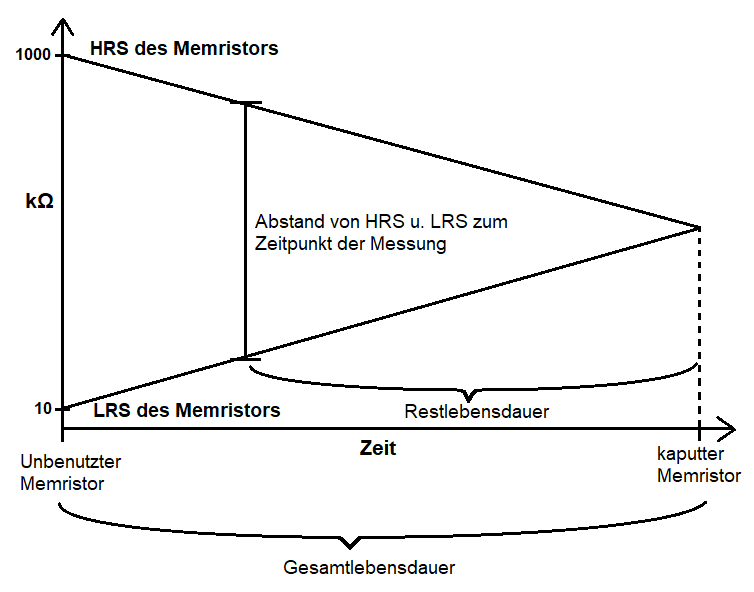
\includegraphics[width=0.7\textwidth]{images/Lebensdauer_Skizze.png}
  \caption{Skizzenhafte Darstellung zur approximierten Berechnung der Restlebensdauer eines Memristors.}
  \label{fig:Lebensdauer_Skizze}
\end{figure}

Da alle Parameter gegeben oder in einem vorherigen Schritt gemessen wurden, kann die Restlebensdauer durch diese Berechnung einfach approximiert werden. Dabei kann für die approximierte Gesamtlebensdauer $t$ jeweils der minimale, typische und maximale Wert aus dem Datenblatt von Knowm~\cite{knowm_comp_2019} verwendet werden. Es gibt also auch drei mögliche approximierte Restlebensdaueren anhand dieser drei Werte. Die Note wird nur beeinflusst, wenn die Restlebensdauer sehr kurz ist. Als Wert, ab welchem die Note beeinflusst wird, wurde hierbei $\frac{1}{10}$ der minimalen gesamten Lebensdauer gewählt, da dabei bereits $90\%$ der Schreibzyklen des Memristors durchlaufen wurden und er somit im worst-case keine sehr lange Laufzeit mehr vorzuweisen hat. Die approximierte Restlebensdauer wird immer nach der Angabe der Note in einem Tripel aus maximaler, typischer und minimaler Restlebensdauer ausgegeben, damit der Nutzer unabhängig zur Note eine Aussage über diese erhält.

Wurde im letzten Schritt die Restlebensdauer approximiert, so kann nun eine Gesamtnote angegeben werden. Diese berechnet sich, wie bereits im vorherigen Kapitel dargestellt wurde, wie folgt:
\begin{align}
  &(\text{f-Grade } + \text{ t-Grade } + \text{ s-Grade})/3 + L\\
  &\text{mit } L =
  \begin{cases}
      1, &\text{ wenn Restlebensdauer < 10\% der Gesamtlebensdauer} \\
      0, &\text{ sonst}
  \end{cases}\nonumber
\end{align}

\section{Die Ausgabe des Programms}

Dieser Abschnitt wird sich mit der Ausgabe des Programms beschäftigen. Wie in Abbildung~\ref{fig:Ausgabe} zu erkennen ist, ist die Ausgabe in mehrere Teile aufgeteilt. Während der Messungen und der Berechnungen der Implementierung wird nach jedem der fünf großen Schritte in der Ausgabe eine Mitteilung geschickt, dass der Schritt abgeschlossen wurde. Im folgenden Kapitel~\ref{sec:Chapter5} wird die Laufzeit des Programms thematisiert. Dabei wird gezeigt, dass es teilweise zu längeren Laufzeiten kommen kann. Damit der Nutzer nicht das Gefühl bekommt, dass nichts passiert, wird deshalb nach jedem Schritt eine Mitteilung über die Konsole geschickt, dass dieser Schritt abgeschlossen ist.

\begin{figure}
  \centering
    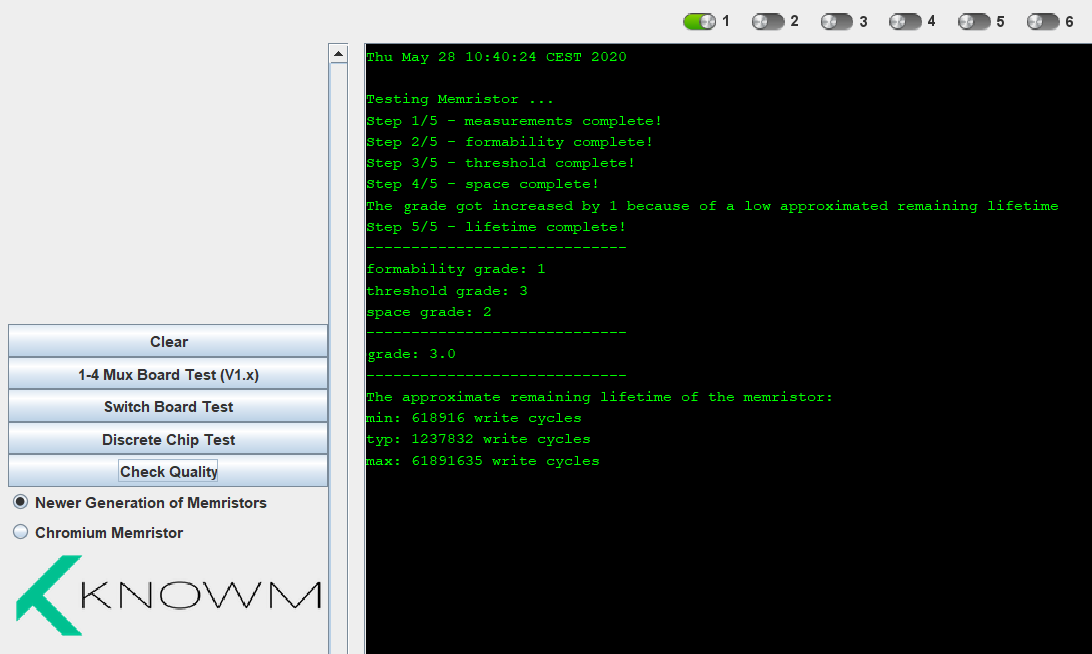
\includegraphics[width=0.95\textwidth]{images/Beispiel_Ausgabe.png}
  \caption{Beispielhafte Ausgabe des implementierten Programms für einen Memristor aus Wolfram der neuen Generation.}
  \label{fig:Ausgabe}
\end{figure}

Sind alle fünf Schritte vollendet, kommt es zu der eigentlichen Ausgabe des Programms. Durch Trennlinien wird der erste Teil der Ausgabe mit der Ausgabe der drei Teilnoten \glqq f-grade\grqq\,(formability grade), \glqq t-grade\grqq\,(threshold grade) und \glqq s-grade\grqq\,(space grade) getrennt. Nach der Ausgabe dieser Teilnoten wird erneut durch Trennlinien die Gesamtnote \glqq Grade\grqq\,ausgegeben. Ganz zum Schluss werden die approximierte minimale, typische und maximale Restlebensdauer in Schreibzyklen ausgegeben. Unterschreitet die minimale Restlebensdauer 10\% der minimalen Gesamtlebensdauer, so wird nach der Beendigung des vierten Schrittes zu Beginn schon eine Mitteilung gesendet, dass die Gesamtnote um eine Note verschlechtert wurde, da die approximierte Restlebensdauer zu niedrig ist.



%\begin{itemize}
%  \item Implementierung nach Konzept aus Abbildung~\ref{fig:Notengenerierung}
%  \item 1. Formbarkeit:
%  \begin{itemize}
%    \item Hysterese auslesen, Punkte analysieren (ist eine Hysterese vorhanden?)
%    \item 4-5 verschiedene Amplituden, Offsets, Frequenzen durchtesten und Unterschiede analysieren (Ausmaß an Formbarkeit)
%  \end{itemize}
%  \item 2. Threshold:
%  \begin{itemize}
%    \item Hysterese analysieren und Threshold auslesen
%  \end{itemize}
%  \item 3. Speichergröße:
%  \begin{itemize}
%    \item da der Threshold bekannt ist, muss jetzt in einen möglichst maximalen Widerstand des Memristors gewechselt werden. (Umkehren des Memristors möglicherweise verwendbar)
%    \item daraufhin soweit den Widerstand des Memristors senken, bis er nicht mehr weniger wird oder ein minimaler Widerstand erreicht wird (10-15kOhm erste Einschätzung)
%  \end{itemize}
%  \item 4. Lebensdauer:
%  \begin{itemize}
%    \item in der Folge der Speichergrößenbestimmung wird maximaler und minimaler Widerstand bestimmt.
%    \item Differenz zwischen den beiden berechnen
%    \item eine Funktion aufstellen anhand welcher eine Restlebensdauer approximiert werden kann
%  \end{itemize}
%  \item 5. Temperatur:
%  \begin{itemize}
%    \item unbekannt, ob relavant oder überhaupt möglich über Digilent Discovery Board messbar
%    \item wenn Funktion vorhanden -> Messreihe über Temperaturen von allen funktionierenden Memristoren nach Ablauf der vorherigen Schritten
%    \item gibt es Unterschiede ->  >>zu hoch<< definieren
%  \end{itemize}
%\begin{table}
%  \begin{tabular}{|c|c|c|c|}
%    \hline
%    \textbf{Note} & \textbf{Formbarkeit} & \textbf{Threshold} & \textbf{Speichergröße}\\\hline
%     1             & sehr formbar         & > 0.1 \& <= 0.3     & 6 Bit (>= 64 Zustände)\\\hline
%     2             & formbar              & > 0.3 \& <= 0.5     & 5 Bit (>= 32 Zustände)\\\hline
%     3             & wenig formbar        & > 0.5 \& <= 0.7     & 4 Bit (>= 16 Zustände)\\\hline
%     4             & kaum formbar         & > 0.7 \& <= 0.8     & 3 Bit (>= 8 Zustände) \\\hline
%  \end{tabular}
%  \caption{Notenvergabe Tabelle}
%  \label{tab:Note}
%\end{table}
%\end{itemize}
